



\documentclass[first=dgreen,second=purple,logo=yellowexc]{aaltoslides}
%\documentclass{aaltoslides} % DEFAULT
%\documentclass[first=purple,second=lgreen,logo=redque,normaltitle,nofoot]{aaltoslides} % SOME OPTION EXAMPLES





% input encode
\usepackage[utf8]{inputenc}


%\usepackage[T1]{fontenc}
%\usepackage{lastpage}
%\usepackage{multirow}
%\usepackage{colortbl}
%\usepackage{comment}
%\usepackage{bm}
%\usepackage{natbib}


% Lipsum package generates bullshit
%\usepackage{lipsum}

% Set the document languages
%\usepackage[finnish,swedish,english]{babel}

% nomenclature
%\usepackage[intoc]{nomencl}

% math
\usepackage{amsmath}

% bibliograph
%\usepackage{natbib}

% For algorithms
\usepackage{algorithm}
\usepackage{algorithmic}

% math font
\usepackage{amsfonts}

% theory
%\usepackage{amsthm}

% double bracket
\usepackage{stmaryrd}

% special math symbol
\usepackage{amssymb}

% use enumerate environment
%\usepackage{enumitem}

% use \url \hyperref, make reference clickable
\usepackage{hyperref}

% use lastpage to inde
\usepackage{lastpage}



%-------------------
%
% set
%
%-------------------
\newcommand{\Acal}{\mathcal{A}}
\newcommand{\Bcal}{\mathcal{B}}
\newcommand{\Ccal}{\mathcal{C}}
\newcommand{\Dcal}{\mathcal{D}}
\newcommand{\Ecal}{\mathcal{E}}
\newcommand{\Fcal}{\mathcal{F}}
\newcommand{\Gcal}{\mathcal{G}}
\newcommand{\Hcal}{\mathcal{H}}
\newcommand{\Ical}{\mathcal{I}}
\newcommand{\Jcal}{\mathcal{J}}
\newcommand{\Kcal}{\mathcal{K}}
\newcommand{\Lcal}{\mathcal{L}}
\newcommand{\Mcal}{\mathcal{M}}
\newcommand{\Ncal}{\mathcal{N}}
\newcommand{\Ocal}{\mathcal{O}}
\newcommand{\Pcal}{\mathcal{P}}
\newcommand{\Qcal}{\mathcal{Q}}
\newcommand{\Rcal}{\mathcal{R}}
\newcommand{\Scal}{\mathcal{S}}
\newcommand{\Tcal}{\mathcal{T}}
\newcommand{\Ucal}{\mathcal{U}}
\newcommand{\Vcal}{\mathcal{V}}
\newcommand{\Wcal}{\mathcal{W}}
\newcommand{\Xcal}{\mathcal{X}}
\newcommand{\Ycal}{\mathcal{Y}}
\newcommand{\Zcal}{\mathcal{Z}}

\newcommand{\RR}{\mathbb{R}}
\newcommand{\ZZ}{\mathbb{Z}}

%-------------------
%
% vector
%
%-------------------
\newcommand{\va}{\mathbf {a}}
\newcommand{\vb}{\mathbf {b}}
\newcommand{\vc}{\mathbf {c}}
\newcommand{\vd}{\mathbf {d}}
\newcommand{\ve}{\mathbf {e}}
\newcommand{\vf}{\mathbf {f}}
\newcommand{\vg}{\mathbf {g}}
\newcommand{\vh}{\mathbf {h}}
\newcommand{\vi}{\mathbf {i}}
\newcommand{\vj}{\mathbf {j}}
\newcommand{\vk}{\mathbf {k}}
\newcommand{\vl}{\mathbf {l}}
\newcommand{\vm}{\mathbf {m}}
\newcommand{\vn}{\mathbf {n}}
\newcommand{\vo}{\mathbf {o}}
\newcommand{\vp}{\mathbf {p}}
\newcommand{\vq}{\mathbf {q}}
\newcommand{\vr}{\mathbf {r}}
\newcommand{\vs}{\mathbf {s}}
\newcommand{\vt}{\mathbf {t}}
\newcommand{\vu}{\mathbf {u}}
\newcommand{\vv}{\mathbf {v}}
\newcommand{\vw}{\mathbf {w}}
\newcommand{\vx}{\mathbf {x}}
\newcommand{\vy}{\mathbf {y}}
\newcommand{\vz}{\mathbf {z}}
\newcommand{\vmu}{\mathbf {\mu}}
\newcommand{\valpha}{\mathbf {\alpha}}
\newcommand{\vlambda}{\mathbf {\lambda}}
\newcommand{\vAlpha}{\mathbf {\Alpha}}
\newcommand{\vbeta}{\mathbf {\beta}}
\newcommand{\vBeta}{\mathbf {\Beta}}
\newcommand{\vgamma}{\mathbf {\gamma}}
\newcommand{\vGamma}{\mathbf {\Gamma}}
\newcommand{\vdelta}{\mathbf {\dalta}}
\newcommand{\vDelta}{\mathbf {\Dalta}}
\newcommand{\vone}{\mathbf {1}}
\newcommand{\vzero}{\mathbf {0}}
\newcommand{\vell}{\mathbf {\ell}}
\newcommand{\vxi}{\mathbf{\xi}}
\newcommand{\vphi}{\mathbf{\phi}}
\newcommand{\vPhi}{\mathbf{\Phi}}

%-------------------
%
% math operation
%
%-------------------
\newcommand{\argmax}{\textbf{argmax}}
\newcommand{\argmin}{\textbf{argmin}}
\newcommand{\sign}{\textbf{sign}}
\newcommand{\maximize}{\textbf{max}}
\newcommand{\minimize}{\textbf{min}}
\newcommand{\argkmax}{\textbf{argkmax}}
\newcommand{\argkmin}{\textbf{argkmin}}
\newcommand{\kmaximize}{\textbf{kmax}}
\newcommand{\kminimize}{\textbf{kmin}}
\newcommand{\st}{\textbf{s.t.}}
\newcommand{\set}[1]{\{ #1 \}}
%\newcommand{\ind}[1]{{\llbracket #1 \rrbracket}}
\newcommand{\ind}[1]{\mathbf{1}_{\{#1\}}}
\newcommand{\norm}[1]{\left|\left| #1 \right|\right|}
\newcommand{\ip}[2]{\langle #1, #2 \rangle}
\newcommand{\var}{\textbf{Var}}
\newcommand{\E}{\textbf{E}}
\newcommand{\exponential}[1]{e^{ #1 }}


\newcommand{\Gva}{G_{\va}}
%-------------------
%
% writings
%
%-------------------
\newcommand{\eqdef}{\overset{{\rm \mbox{\tiny def}}}{=}}
\newcommand{\sbf}[1]{\boldsymbol{#1}}
\newcommand{\mbf}[1]{\mathbf{#1}} 
\newcommand{\etal}{{\em et al.}}

\newcommand{\svmstruct}{{\sc ssvm}}
\newcommand{\mmmn}{{\sc m$^3$n}}
\newcommand{\svm}{{\sc svm}}
\newcommand{\mmcrf}{{\sc mmcrf}}
\newcommand{\smo}{{\sc smo}}
\newcommand{\crf}{{\sc crf}}
\newcommand{\nphard}{$\Ncal\Pcal$-hard}
\newcommand{\nphardness}{$\Ncal\Pcal$-hardness}
\newcommand{\iis}{{\sc iis}}
\newcommand{\memm}{{\sc memm}}
\newcommand{\lr}{{\sc lr}}
\newcommand{\svmlight}{{\sc svmlight}}
\newcommand{\libsvm}{{\sc libsvm}}
\newcommand{\svmcascade}{{\sc svmcascade}}
\newcommand{\adaboost}{{\sc adaboost}}
\newcommand{\adaboostmh}{{\sc adaboost.mh}}
\newcommand{\bagging}{{\sc bagging}}
\newcommand{\vrtree}{{\sc vr-tree}}
\newcommand{\deepboosting}{{\sc deepboosting}}
\newcommand{\loo}{{\sc loo}}
\newcommand{\mtl}{{\sc mtl}}
\newcommand{\sdp}{{\sc sdp}}
\newcommand{\iqp}{{\sc iqp}}
\newcommand{\qp}{{\sc qp}}
\newcommand{\daggraph}{{\sc dag}}
\newcommand{\lp}{{\sc lp}}

\newcommand{\hatf}{{\hat{f}}}
\newcommand{\p}{\sc p}
\newcommand{\n}{\sc n}
\newcommand{\pp}{\sc pp}
\newcommand{\pn}{\sc pn}
\newcommand{\nn}{\sc nn}
\newcommand{\maxcut}{{\sc max-cut}}
\newcommand{\greedy}{{\sc greedy}}
\newcommand{\kernelcascade}{{\sc kernel cascade}}
\newcommand{\netrate}{{\sc netrate}}
\newcommand{\netinf}{{\sc netinf}}
\newcommand{\spin}{{\sc spin}}
\newcommand{\vI}{\mathbf{I}}
\newcommand{\tp}{^{\intercal}}
\newcommand{\mve}{{\sc mve}}
\newcommand{\amm}{{\sc amm}}
\newcommand{\mam}{{\sc mam}}
\newcommand{\rta}{{\sc rta}}
\newcommand{\lasso}{{\sc lasso}}
\newcommand{\mle}{{\sc mle}}
\newcommand{\map}{{\sc map}}
\newcommand{\rbf}{{\sc rbf}}
\newcommand{\mlknn}{{\sc ml-knn}}
\newcommand{\knn}{{\sc knn}}
\newcommand{\iblr}{{\sc iblr}}
\newcommand{\cc}{{\sc cc}}
\newcommand{\pcc}{{\sc pcc}}
\newcommand{\ecc}{{\sc ecc}}
\newcommand{\br}{{\sc br}}
\newcommand{\corrlog}{{\sc corrlog}}
\newcommand{\ilgs}{{\sc ilgs}}
\newcommand{\ilrs}{{\sc ilrs}}
\newcommand{\cpp}{{\sc c}}
\newcommand{\matlab}{{\sc matlab}}
\newcommand{\openmp}{{\sc openmp}}
\newcommand{\python}{{\sc python}}
\newcommand{\cvx}{{\sc cvx}}
\newcommand{\lda}{{\sc lda}}
\newcommand{\kkt}{{\sc k.k.t}}
\newcommand{\lbp}{{\sc lbp}}
\newcommand{\anova}{{\sc anova}}

\renewcommand{\algorithmicrequire}{\textbf{Input:}}
\renewcommand{\algorithmicensure}{\textbf{Output:}}



\newcommand{\Upsilonb}{\pmb \Upsilon}
\newcommand{\phib}{\pmb \phi}
\newcommand{\psib}{\pmb \psi}
\newcommand{\varphib}{\pmb \varphi}
\newcommand{\phibh}{\hat\phib}
\newcommand{\psibh}{\hat \psib}
\newcommand{\vYcal}{\pmb \Ycal}
\newcommand{\vXcal}{\pmb \Xcal}
\newcommand{\vFcal}{\pmb \Fcal}
%-------------------
%
% others
%
%-------------------




%\newtheorem{definition}{Definition}
%\newtheorem{theory}{Theory}
%\newtheorem{lemma}{Lemma}

















\title{Transporter protein classification by structured prediction and multiple kernel }
\author{Hongyu Su}



\institute[ICS]{
Helsinki Institute for Information Technology HIIT\\
Department of Computer Science\\
Aalto University
}

\aaltofootertext{Transporter classification}{\today}{\arabic{page}}


\date{ \today} %\date{Version 1.0, \today}

\iffalse
\AtBeginSection[]
{
  \begin{frame}<beamer>{Outline}
    \tableofcontents[currentsection,subsection]
  \end{frame}
}
\fi




%--------------------------------
%
% document
%
%--------------------------------

\begin{document}

\aaltotitleframe
\footnotesize

\begin{frame}{Motivation}
	\begin{itemize}
		\item Membrane transporter proteins cover $10\%$ proteins in a cell.
		\item An accurate classification model can help in
		\begin{itemize}\footnotesize
			\item studying comparative and functional genomics
			\item probing metabolic processes
			\item developing new therapeutic targets
			\item identifying pharmacologically proteins 
		\end{itemize}
		\item Transporter protein classification \tc\ is a hierarchical system of thousands of classes.
		\item By predicting the whole \tc\ system, we implicitly predict
		\begin{itemize}\footnotesize
			\item mode of actions
			\item energy coupling mechanism
			\item phylogenetic group
			\item substrate specificity
		\end{itemize}
		\item Additionally, we would also benefit from the relationship between classes (class-subclasses, different level of granularities).
		\item The prediction task: input is a transporter protein sequence; output is the corresponding \tc.
	\end{itemize}
\end{frame}

\begin{frame}{Notations}
	\begin{itemize}\footnotesize
		\item Training examples come in pairs $(\vx,\vy)\in\vXcal\times\vYcal$.
		\item $\vXcal$ is an arbitrary input space.
		\item $\vYcal$ is an output space of a collection of $\ell$-dimensional {\em multilabels}.
		\begin{align*}\footnotesize
			\vy=(y_1,\cdots,y_{\ell})\in\vYcal.
		\end{align*}
		\item $y_i$ is a {\em microlabel} and $y_i\in\{+1,-1\}$.
		\item $\vx$ is a protein sequence, $y_i$ is a function class, $\ell=3145$.
		\item We are given a set of $m$ training examples $\{(\vx_i,\vy_i)\}_{i=1}^m$.
		%\item An arbitrary pair $(\vx_i,\vy),\,\vy_\in\vYcal$ is called pseudo-example.
		\item Each example $(\vx,\vy)$ is mapped into a joint feature space $\phib(\vx,\vy)$.
		\item $\vw$ is the weight vector operates in the joint feature space.
		\item Define a linear score function $F(\vw,\vx,\vy) = \ip{\vw}{\phib(\vx,\vy)}$.
		\item $\vw$ ensures that example $\vx_i$ with correct multilabel $\vy_i$ achieves higher score than with any other incorrect multilabel $\vy'\in\vYcal$.
	\end{itemize}
\end{frame}

\begin{frame}{Prediction}
	\begin{itemize}
		\item The prediction $\vy_{\vw}(\vx)$ of an input $\vx$ is the multilabel $\vy$ that maximizes the score function 
		\begin{align}\footnotesize
			\vy_{\vw}(\vx) = \underset{\vy\in\vYcal}{\argmax}\,\ip{\vw}{\phib(\vx,\vy)}. \label{inference}
		\end{align}
		\item Search space is exponential in size, $|\vYcal|=2^{\ell}$.
		\item (\ref{inference}) is called {\em inference} problem which is \nphard\ for most output feature maps.
		\item Often, we want a feature map in which the inference can be solved with a polynomial algorithm, e.g., dynamic programming.
	\end{itemize}
\end{frame}

\begin{frame}{TC hierarchy as the output graph}
	\begin{itemize}\footnotesize
		\item Transporter classification (\tc) system is a hierarchical system.
		\begin{center}
			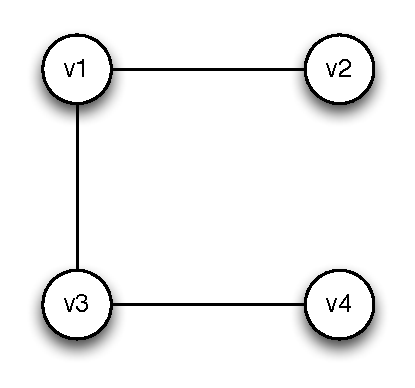
\includegraphics[scale=0.3]{./outputgraph.pdf}
		\end{center}
		\item A vertex $v_i\in V$ corresponds to a microlabel $y_i$ (function class).
		\item An edge $(v_i,v_j)\in E$ corresponds to class-subclass of the microlabel $y_i$ and $y_j$.
		\item We assume that the joint feature map $\phib$ is a potential function on the \tc\ hierarchy $G=(E,V)$.
		\item $\varphib(\vx)\in\RR^d$ is the input feature map, e.g., N-gram feature of a sequence.
		\item $\psib(\vy)\in\RR^{4|E|}$ is the output feature map which maps the multilabel $\vy$ into a collection of edges and labels
		\begin{align*}\footnotesize
			\varphib(\vy) = (\vone_{(\vy_e=u_{e})})_{e,u_e}, e\in E,u_e\in\{-1,+1\}^2.
		\end{align*}
	\end{itemize}
\end{frame}

\begin{frame}{An example of $\psib(\vy)$}
	\begin{itemize}\footnotesize
		\item Given \tc\ hierarchy $G=(E,V)$
		\begin{center}
			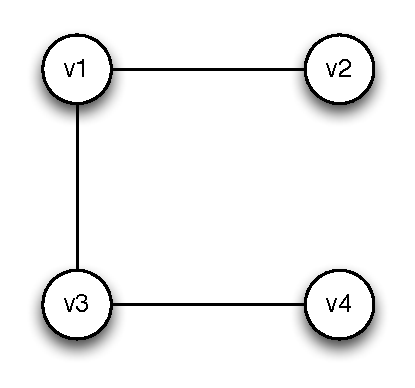
\includegraphics[scale=0.3]{./outputgraph.pdf}
		\end{center}
		\item Multilabel $\vy$
		\begin{align*}
			\vy&=(y_1,y_2,y_3,y_4,y_5)=(+1,-1,+1,+1,-1)
		\end{align*}
		\item Output feature map $\psib(\vy)$
		\begin{align*}\footnotesize
			\psib(\vy) &= ( \underbrace{\underbrace{0}_{--}, \underbrace{0}_{-+}, \underbrace{0}_{+-}, \underbrace{1}_{++},}_{(v_1,v_3)} 
			\underbrace{\underbrace{0}_{--}, \underbrace{0}_{-+}, \underbrace{1}_{+-}, \underbrace{0}_{++},}_{(v_1,v_2)}\cdots)
		\end{align*}
	\end{itemize}
\end{frame}

%
\begin{frame}{Joint feature map $\phib(\vx,\vy)$}
	\begin{itemize}\footnotesize
		\item The joint feature is the Kronecker product of $\varphib(\vx)$ and $\psib(\vy)$
		\begin{align*}\footnotesize
			\phib(\vx,\vy) = (\phib_e(\vx,\vy))_{e\in E}=(\varphib(\vx)\otimes\psib_e(\vy_e))_{e\in E}.
		\end{align*}
		\begin{center}
			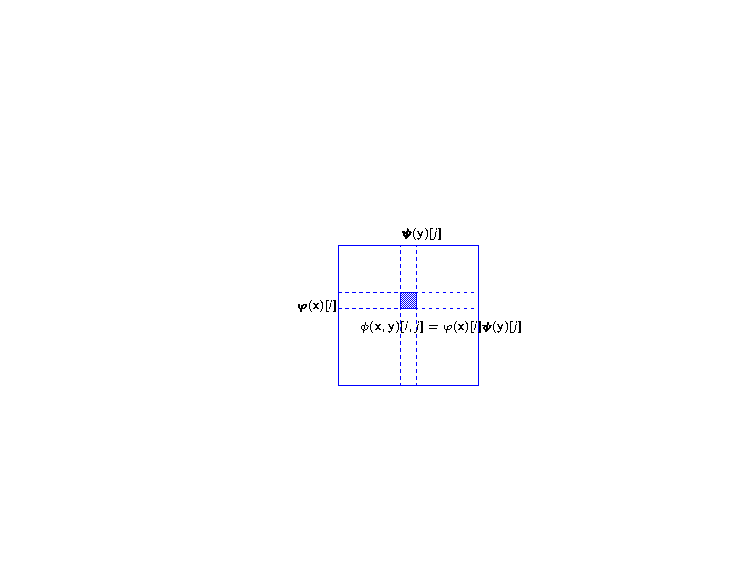
\includegraphics[scale = 1]{./tensor_label.pdf}
		\end{center}
		\item The score function can be factorized by the output graph $G$
		\begin{align*}
			F(\vw,\vx,\vy) = \ip{\vw}{\phib(\vx,\vy)} = \sum_{e\in E}\ip{\vw_e}{\phib_e(\vx,\vy_e)}.
		\end{align*}
	\end{itemize}
\end{frame}

\begin{frame}{Search space reduction}
	\begin{itemize}
		\item Recall the inference problem
		\begin{align*}\footnotesize
			\vy_{\vw}(\vx) = \underset{\vy\in\vYcal}{\argmax}\,\ip{\vw}{\phib(\vx,\vy)}.
		\end{align*}
		\item Search space $|\vYcal| = 2^{\ell}$.
		\item Given \tc\ hierarchy $G=(E,V)$
		\begin{center}
			\only<1>{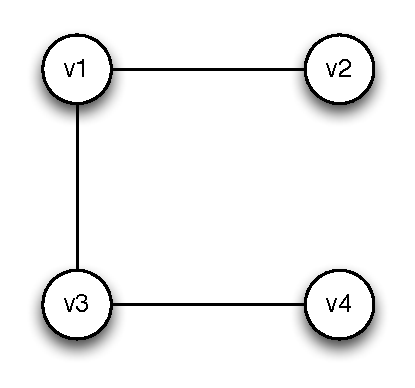
\includegraphics[scale=0.3]{./outputgraph.pdf}}
			\only<2>{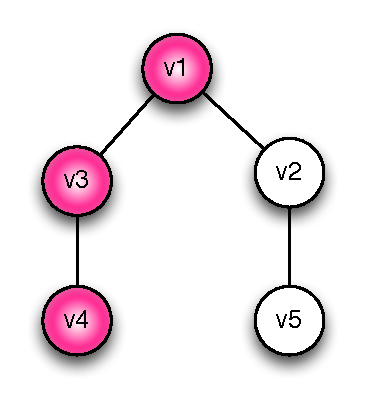
\includegraphics[scale=0.3]{./validlabel1.pdf}}
			\only<3>{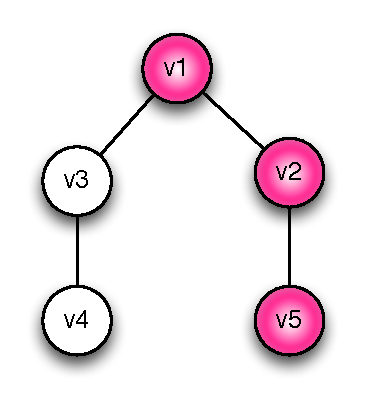
\includegraphics[scale=0.3]{./validlabel2.pdf}}
		\end{center}
		\item Valid multilabels defined by the \tc\ hierarchy
		\begin{align*}
			\vy&=(y_1,y_2,y_3,y_4,y_5)=(+1,-1,+1,+1,-1),\\
			\vy&=(y_1,y_2,y_3,y_4,y_5)=(+1,+1,-1,-1,+1).
		\end{align*}
		\item Search space reduction $|\vYcal| = |V_{\text{leave}}|$.
	\end{itemize}
\end{frame}

\begin{frame}{Optimization problem}
	\begin{itemize}
		\item Solve the following optimization problem to learn $\vw$
		\begin{align*}
			\underset{\vw,\xi_i}{\minimize} & \quad \frac{1}{2}\norm{\vw}_2^2 + C\sum_{i=1}^{m}\xi_i 	\\
			\st & \quad \ip{\vw}{\phib(x_i,\vy_i)} - \underset{\vy\in\Ycal/\vy_i}{\maximize} \ip{\vw}{\phib(x_i,\vy)} \geq \ell(\vy_i,\vy) -  \xi_k,  \\
			& \quad \xi_i\ge0\, , \forall\ i \in \set{1,\dots,m},
		\end{align*}
		\item The impact of the constraints of the above optimization problem is to push the score of input $\vx_i$ with correct multilabel $\vy_i$ above the scores of all competing multilabels $\vy\in\Ycal/\vy_i$. 
		\item The slack parameters $\xi_i$ is used to relax the constraints so that a feasible solution can always be found.
		\item $C$ is the margin slack parameter that controls the amount of regularization in the model.
		\item The objective minimizes the $L_2$-norm of the weights and the slacks allocated to the training data which is equivalent to maximizing the margin subject to allowing some data to be outliers.
	\end{itemize}
\end{frame}


\begin{frame}{Feature extraction}
	\begin{itemize}
		\item \blast\ features
			\begin{itemize}\footnotesize
				\item Identify database sequences that are similar to a query sequence via \blast\ search.
				\item `Similarity' is defined as \blast\ score (statistically significant matches).
				\item In practice, we build a sequence database with all \tcdb\ sequences.
			\end{itemize}
		\item Features computed from {{\interproscan}}
		\begin{itemize}\footnotesize
			\item Identify sequence signatures via scanning many signature databases.
			\item $18$ databases of $3$ `big categories': {\purple Families, domains, sites, repeats}; {\pink structural domain}; {\red other sequence features}.
		\end{itemize}
		\item Position-specific-score-matrix (\pssm)
		\begin{itemize}\footnotesize
			\item \href{http://www3.imperial.ac.uk/pls/portallive/docs/1/5037998.RPS}{\rpsblast}: identify sequence profiles via scanning $8$ profile database, profile is defined by \pssm.
			\item \href{http://www.ncbi.nlm.nih.gov/books/NBK2590/}{\psiblast}: search a profile against a sequence database
			\begin{enumerate}[(a)]\footnotesize
				\item build a \pssm\ profile for a query sequence.
				\item {\red search a profile against the database} or {\purple compute similarity of two profiles}.
			\end{enumerate}
		\end{itemize}
	\end{itemize}
\end{frame}


\begin{frame}{Summary of data}
	\begin{itemize}
		\item Number of proteins $12515$, number of classes $3145$.
		\item \blast\ features: similarity matrix in which elements are \blast\ scores.
		\item \interproscan\ features\\
		{\scriptsize\begin{tabular}{|c|c||c|c||c|c|}\hline
		 Type & Dim & Type & Dim & Type & Dim  \\ \hline
		 Protein Domain & 145 & Hapmap & 209 & SMART & 240 \\
		 Protein Family & 512 & PRINTS & 579 & Panther & 4070 \\
		 Gene3D & 611 & PIRSF & 283 & PfamA & 2025 \\
		 Prosite Profile & 282  & TIGRFAM & 769 & Prosite Patterns & 285\\
		 Coil & 1 & TMHMM& 1& Phobius &7 \\
		 SignalP1& 2& SignalP2 & 2 & SignalP3 & 1\\\hline
		\end{tabular}}
		\item \pssm\ features (size of DB)\\
		{\scriptsize\begin{tabular}{|c|c||c|c|}\hline
		 Type & Dim & Type & Dim \\ \hline
		 CDD & 47363 & Pfam & 14837\\
		 COG & 4825  & KOG  & 4875 \\
		 SMART & 1013 & PRK & 10885 \\
		 TiGRFAM & 4488  & CDD NCBI & 11273\\ \hline
		\end{tabular}}
	\end{itemize}
\end{frame}

\begin{frame}{Multiple kernel learning (\mkl)}
	\begin{itemize}
		\item A collection of $p$ feature maps $\{\varphi_k(\vx)\}_{k=1}^p$ is on hand.
		\item We use \mkl\ to combine these feature maps.\\
		\item Input kernels $\{K_1,\cdots,K_p\}$ and target kernel $K_{\vy} = YY^{\tp}$.
		\item {\bf Uniform kernel combination (\kunif)}
		\begin{align*}
		    K_{\text{\kunif}}=\sum_{k=1}^{p}\frac{1}{p}K^c_k,
		\end{align*}
		\item {\bf Centred kernel alignment (\kalign)}
		\begin{align*}
			K_{\text{\kalign}}=\sum_{k=1}^{p}\alpha_kK^c_k,\quad \alpha_k = \frac{\ip{K^c_k}{K^{c}_{\vy}}_{F}}{\norm{K^c_k}_F\norm{K_{\vy}^{c}}_F} 
		\end{align*}
		\item {\bf Two stage \mkl\ (\kalignf)}
		\begin{align*}
			K_{\text{\kalignf}}=\sum_{k=1}^{p}\beta_k K^c_k, \quad
			\underset{\beta}{\maximize}\, & \displaystyle \frac{\ip{K_{\text{\kalignf}}^c}{K_{\vy}^c}_F}{\norm{K_{\text{\kalignf}}}_F\norm{K_{\vy}^c}_F},
		    \quad \st\,  \displaystyle \sum_{k=1}^p\beta_k^2=1,  \beta_k\ge0,\,\forall k.
		\end{align*}
	\end{itemize}
\end{frame}

\begin{frame}[allowframebreaks]{Experiments}{\svm\ + single feature map + linear kernel}
	{\scriptsize
	\begin{tabular}{|c|c||c|c||c|c|}\hline
		    &   $F_1$		& 		        & $F_1$        &           & $F_1$        \\ \hline
	Blast   &	{\bf 74.5}	& PIRSF	            & 11.2	& SignalP2	    & 3.6    \\
	Coils   &	03.6	& PRINTS	        & 13.7	& SignalP3	    & 4.1    \\
	Gene3D  &	04.0	& ProDom	        & 03.5	& SMART	        & 7.2    \\
	Hamap   &	05.5	& ProSite Patterns	& 03.0	& SUPERFAMILY	& 14.9    \\
	PANTHER &	42.4	& ProSite Profiles	& 15.6	& GRFAM	        & 22.3    \\
	Pfam	&   38.2	& SignalP1	        & 1.1	& TMHMM	        & 06.8    \\
	Phobius	&   11.7	&                   &       &               & \\\hline			
	\end{tabular}}
	\framebreak
	\begin{figure}
		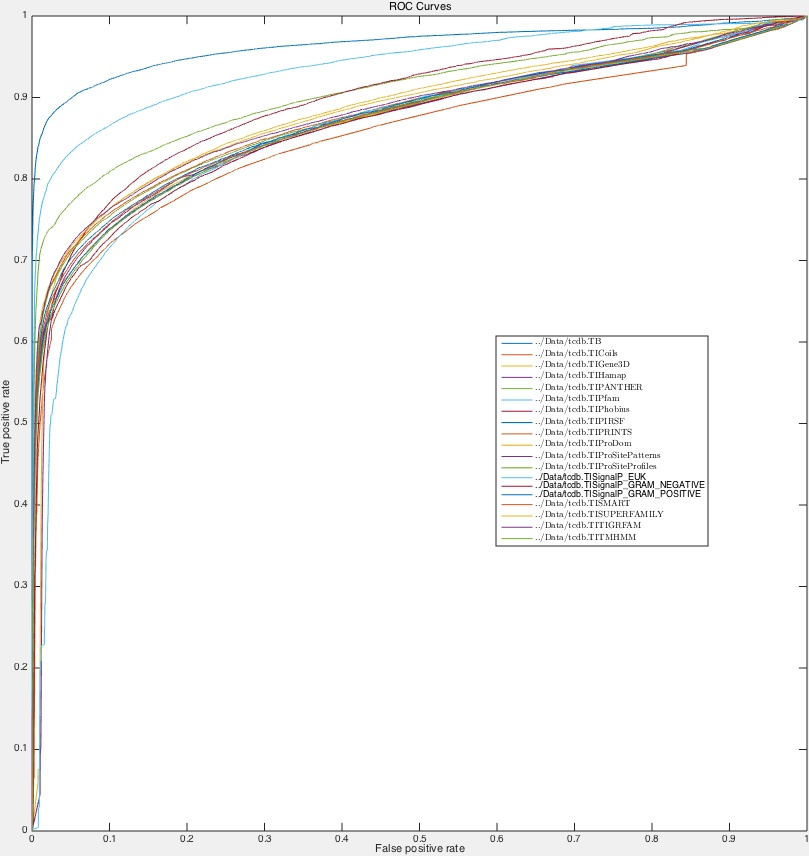
\includegraphics[scale=0.2]{./svmauc.jpg}
	\end{figure}
\end{frame}

\begin{frame}{Experiments}{(\svm, \mmr, \sop) + \mkl\ +  (linear, Gaussian)}
	{\scriptsize
	\begin{tabular}{|p{1cm}|p{0.5cm}|p{0.5cm}p{0.5cm}|p{0.5cm}p{0.5cm}|p{0.5cm}p{0.5cm}|p{0.5cm}p{0.5cm}|} \hline
		& \multicolumn{5}{c|}{$F_1$} & \multicolumn{4}{c|}{$0/1$} \\ \cline{2-10}
		& \multicolumn{3}{c|}{$Linear$} & \multicolumn{2}{c|}{$Gaussian$} & \multicolumn{2}{c|}{$Linear$} & \multicolumn{2}{c|}{$Gaussian$} \\ \cline{2-10}
		& \svm & \mmr & \sop & \mmr & \sop & \mmr & \sop & \mmr & \sop \\ \hline
	\kunif    & 68.3& 35.1 & 71.7 & 79.9&  79.9  & 06.9 & 55.1 & 64.1 &  64.3 \\ 
	\kalign  & 74.6 & 33.9 & 76.9 & 83.0&  82.8  & 05.9 & 58.4 & 68.3 &  68.6 \\
	\kalignf & 79.2 & 50.1 & 80.0 & {\bf 85.4} &  {\it 85.2}  & 21.0 & 62.9 & {\it 72.7}&  {\bf 72.8} \\ \hline
	\end{tabular}}
\end{frame}

\begin{frame}{Discussion}
	\begin{itemize}
		\item Transporter classification \tc\ system is a hierarchical system.
		\item We developed structured output prediction model \sop\ to predict \tc\ given a protein sequence.
		\item Based on \tc, we are able to dramatically reduce the search space from exponential to linear which allows
		\begin{itemize}\footnotesize
			\item Feasible training
			\item Accurate prediction
		\end{itemize}
		\item For each protein sequence, we generate various types of features and apply \mkl\ to merge multiple input feature maps.
		\item The experiment shows that structured prediction approach significantly improves single label classification approach. 
	\end{itemize}
\end{frame}


\iffalse
\begin{frame}[allowframebreaks]{Bibliography}
	%\bibliographystyle{plain}
	\bibliographystyle{apalike}
	\bibliography{example}
\end{frame}
\fi


\end{document}
